\documentclass{beamer}
\usepackage{graphicx}
\usepackage{tikz}
\usetikzlibrary{shapes,arrows}
\usepackage{tikz}
%\usecolortheme{seahorse}
  \setbeamertemplate{footline}[page number]
\usepackage{multirow}
\setbeamertemplate{navigation symbols}{}
\setbeamertemplate{frametitle}[default][center]
\setbeamerfont{frametitle}{shape=\scshape}
\usepackage{color}

\usepackage{csquotes}

\usepackage{xcolor}

\usepackage[flushleft]{threeparttable}

{\title{\textsc{Econ 352 - A Two-Period Model: The Consumption-Savings Decision and Credit Markets} \\ \tiny (See Williamson Ch. 9)}
\author{Trevor S. Gallen}
\date{}
\begin{document}
\renewcommand*{\inserttotalframenumber}{\pageref{lastframe}}


\setbeamertemplate{caption}{\raggedright\insertcaption\par}

\begin{frame}
\titlepage
\end{frame}

\begin{frame}
\frametitle[alignment=center]{Introduction}
\begin{itemize}
\item We've seen some one-period models of Macro
\bigskip
\item Can think about the ``consumption-leisure" or ``intratemporal" tradeoff
\bigskip
\item But one-period model...what about future?  No savings.
\bigskip
\item Having isolated the consumption-leisure tradeoff, we turn to the ``intertemporal" tradeoff:  consume today vs consume tomorrow
\bigskip
\item Just as the wage was a key driver of the intratemporal decision, the real interest rate will be a key driver of the intertemporal
\end{itemize}
\end{frame}

\begin{frame}
\frametitle[alignment=center]{Two-Period Model}
\begin{itemize}
\item Note: while we'll do a two-period model, not much changes when we shift to a 200-period model
\bigskip
\item Assume $N$ consumers, with real income today $y$ and real income tomorrow $y'$, lump-sum taxes today $t$, and lump-sum taxes tomorrow of $t'$.  Letting savings between periods be $s$, the first period's budget constraint is:
$$c+s=y-t$$
\item The next period, savings recieve interest rate $r$ (so total assets are now $(1+r)s$, and the person consumes everything.  Their budget constraint is:
$$c'=y'-t'+(1+r)s$$
\bigskip
\item Note that both equations have savings ($s$) linking them...really the consumer just faces one full lifetime budget constraint
\end{itemize}
\end{frame}

\begin{frame}
\frametitle[alignment=center]{Lifetime Budget Constraint-I}
\begin{itemize}
\item Solving for $s$ in the second-period:
$$s=\frac{c'-y'+t'}{1+r}$$
\item And plugging into the first period's budget constraint: $c+s=y-t$, we get:
$$c+\frac{c'}{1+r}=y+\frac{y'}{1+r}-t-\frac{t'}{1+r}$$
\item We call this the ``lifetime budget constraint" because it's the total of all the income you have to spend over your whole lifetime
\end{itemize}
\end{frame}

\begin{frame}
\frametitle[alignment=center]{Lifetime Budget Constraint-II}
\begin{itemize}
\item Lifetime budget constraint:
$$c+\frac{c'}{1+r}=y+\frac{y'}{1+r}-t-\frac{t'}{1+r}$$
\item The budget constraint is in terms of ``today's dollars" but we could put it in terms of tomorrow's dollars by multiplying by $(1+r)$:
$$(1+r)c+c'=(1+r)y+y'-(1+r)t-t'$$
\item What both are saying is that (when $r>0$) money today is ``more valuable."  Increasing $c$ by one today costs me $1+r$ $c'$ tomorrow.  Decreasing $c'$ by one tomorrow only increases $c$ by $\frac{1}{1+r}$.  Similarly with income!
\bigskip
\item If the budget constraint doesn't make sense, let's give some examples
\end{itemize}
\end{frame}



\begin{frame}
\frametitle[alignment=center]{Lifetime Budget Constraint: Examples}
\begin{itemize}
\item Let's say $y=y'=1$,  $r=0.5$ (50\% interest rate) and $t=t'=0$ for simplicity.
\item Then we have:
$$c+\frac{c'}{1.5}=1+\frac{1}{1+0.5}-0-\frac{0}{1+0.5}$$
\item Or:
$$c=\frac{5}{3}-\frac{2}{3}c'$$
\item If I spent all my money on today $c'=0$, I could consume \$5/3.  This makes sense:  eat my \$1 of income today, take out a loan of \$0.66, and eat that too.  Then when the second period rolls around, I owe \$1, and have \$1 in income, which I use to pay off my debt.
\item If I spend all my money on tomorrow, $c=0$, and I could consume \$2.5.  How?  I save my \$1 of income today, and it becomes \$1.5 tomorrow, when added to my \$1 of income tomorrow, allows me to buy \$2.5 worth of stuff tomorrow.
\end{itemize}
\end{frame}

\begin{frame}
\frametitle[alignment=center]{Consumer's Lifetime Budget Constraint}
\begin{figure}
\centering
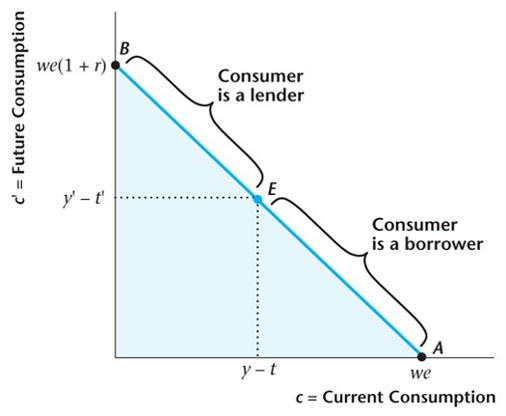
\includegraphics[scale=0.5]{Figures/W_Fig_9pt1.png}
\end{figure}
We have the B.C., now we need preference
\end{frame}

\begin{frame}
\frametitle[alignment=center]{Consumer preferences}
\begin{itemize}
\item Consumers always like more $c$ and more $c'$
\bigskip
\item The consumer likes variety.  Roughly, $c=c'=1$ is preferred to $c=1.99$ and $c'=0.01$.  
\bigskip
\item Both $c$ and $c'$ are normal goods: when lifetime wealth increases, we expect both to increase
\bigskip
\item With this, we can graph indifference curves!
\end{itemize}
\end{frame}

\begin{frame}
\frametitle[alignment=center]{Consumer's Lifetime Budget Constraint}
\begin{figure}
\centering
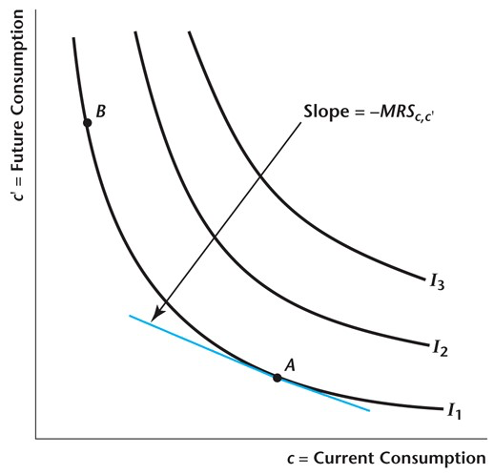
\includegraphics[scale=0.5]{Figures/W_Fig_9pt2.png}
\end{figure}
Just as in the wage example, we will always consume where $MRS=MRT$, in this case: $MRS_{c,c'}=1+r$
\end{frame}

\begin{frame}
\frametitle[alignment=center]{Lenders Consume Less today than Endowment}
\begin{figure}
\centering
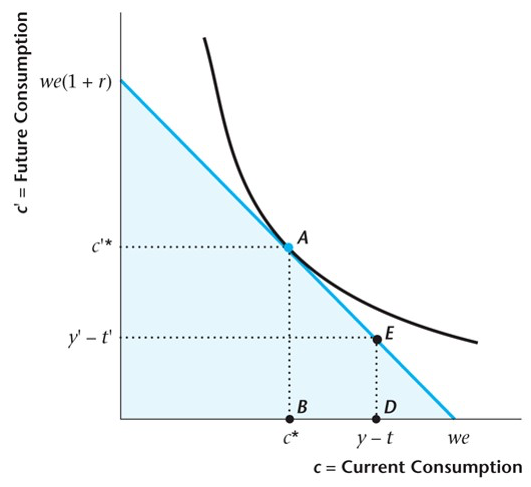
\includegraphics[scale=0.5]{Figures/W_Fig_9pt3.png}
\end{figure}
$$c+\frac{c'}{1+r}=y+\frac{y'}{1+r}-t-\frac{t'}{1+r}$$
\end{frame}

\begin{frame}
\frametitle[alignment=center]{Borrowers Consume More today than Endowment}
\begin{figure}
\centering
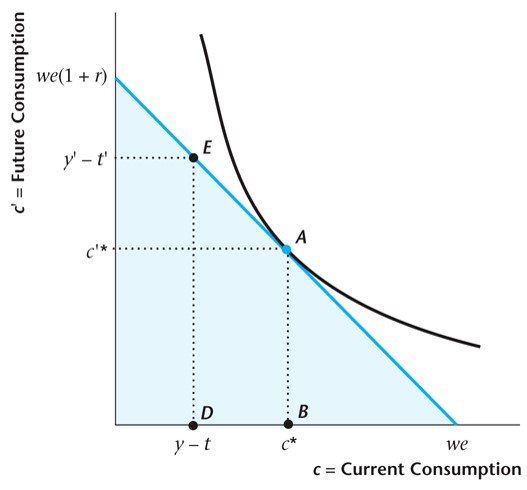
\includegraphics[scale=0.5]{Figures/W_Fig_9pt4.png}
\end{figure}
$$c+\frac{c'}{1+r}=y+\frac{y'}{1+r}-t-\frac{t'}{1+r}$$
\end{frame}

\begin{frame}
\frametitle[alignment=center]{When lifetime today increases, we consume more of all normal goods}
\begin{figure}
\centering
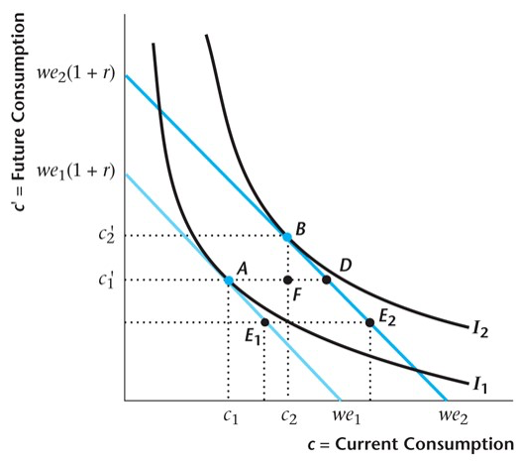
\includegraphics[scale=0.5]{Figures/W_Fig_9pt5.png}
\end{figure}
$$c+\frac{c'}{1+r}=y+\frac{y'}{1+r}-t-\frac{t'}{1+r}$$
note you can't tell if it was $y$ or $y'$ that increased!  Testable implication.
\end{frame}

\begin{frame}
\frametitle[alignment=center]{Predictions}
\begin{itemize}
\item If consumers like to smooth, we predict consumption should be smooth relative to income
\bigskip
\item We can test this with our GDP/consumption graph
\bigskip
\item But first note that durables should probably be with investment
\bigskip
\item Let's take a look
\end{itemize}
\end{frame}

\begin{frame}
\frametitle[alignment=center]{Durables and GDP}
\begin{figure}
\centering
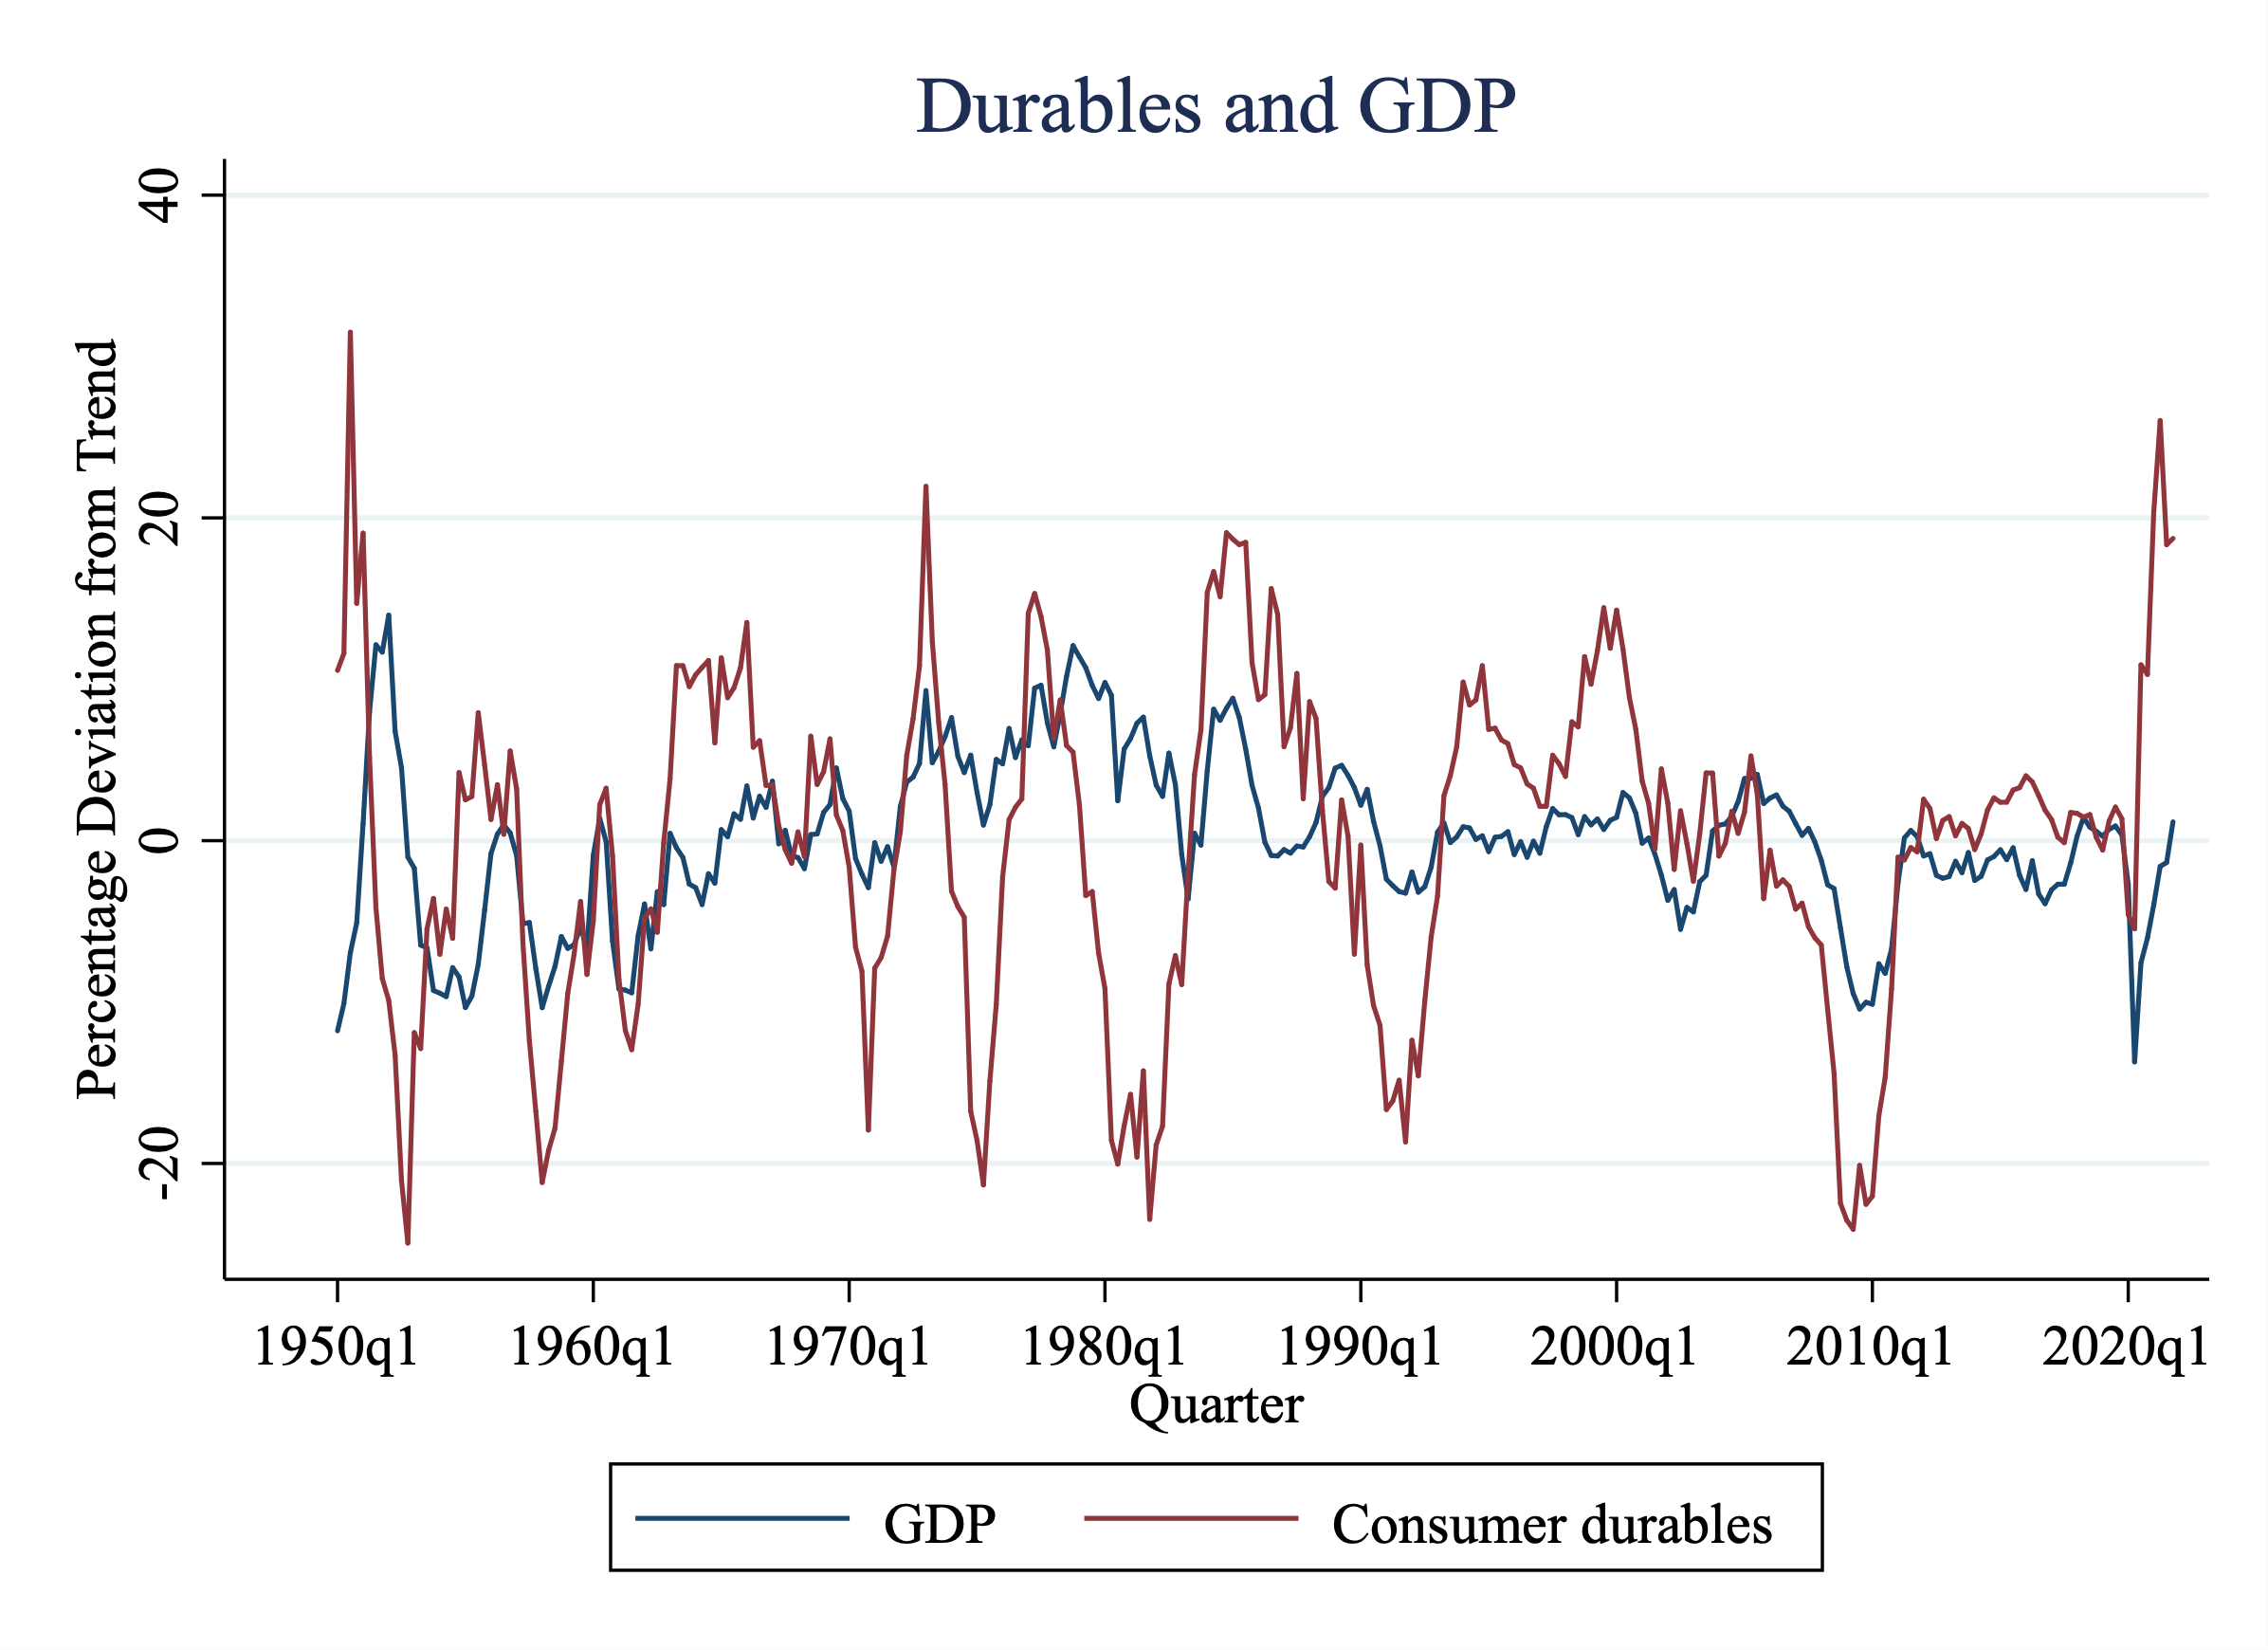
\includegraphics[scale=0.2]{Figures/Fig_9pt6.png}
\end{figure}
Durables, a form of investment/saving, are volatile
\end{frame}

\begin{frame}
\frametitle[alignment=center]{Durables and GDP}
\begin{figure}
\centering
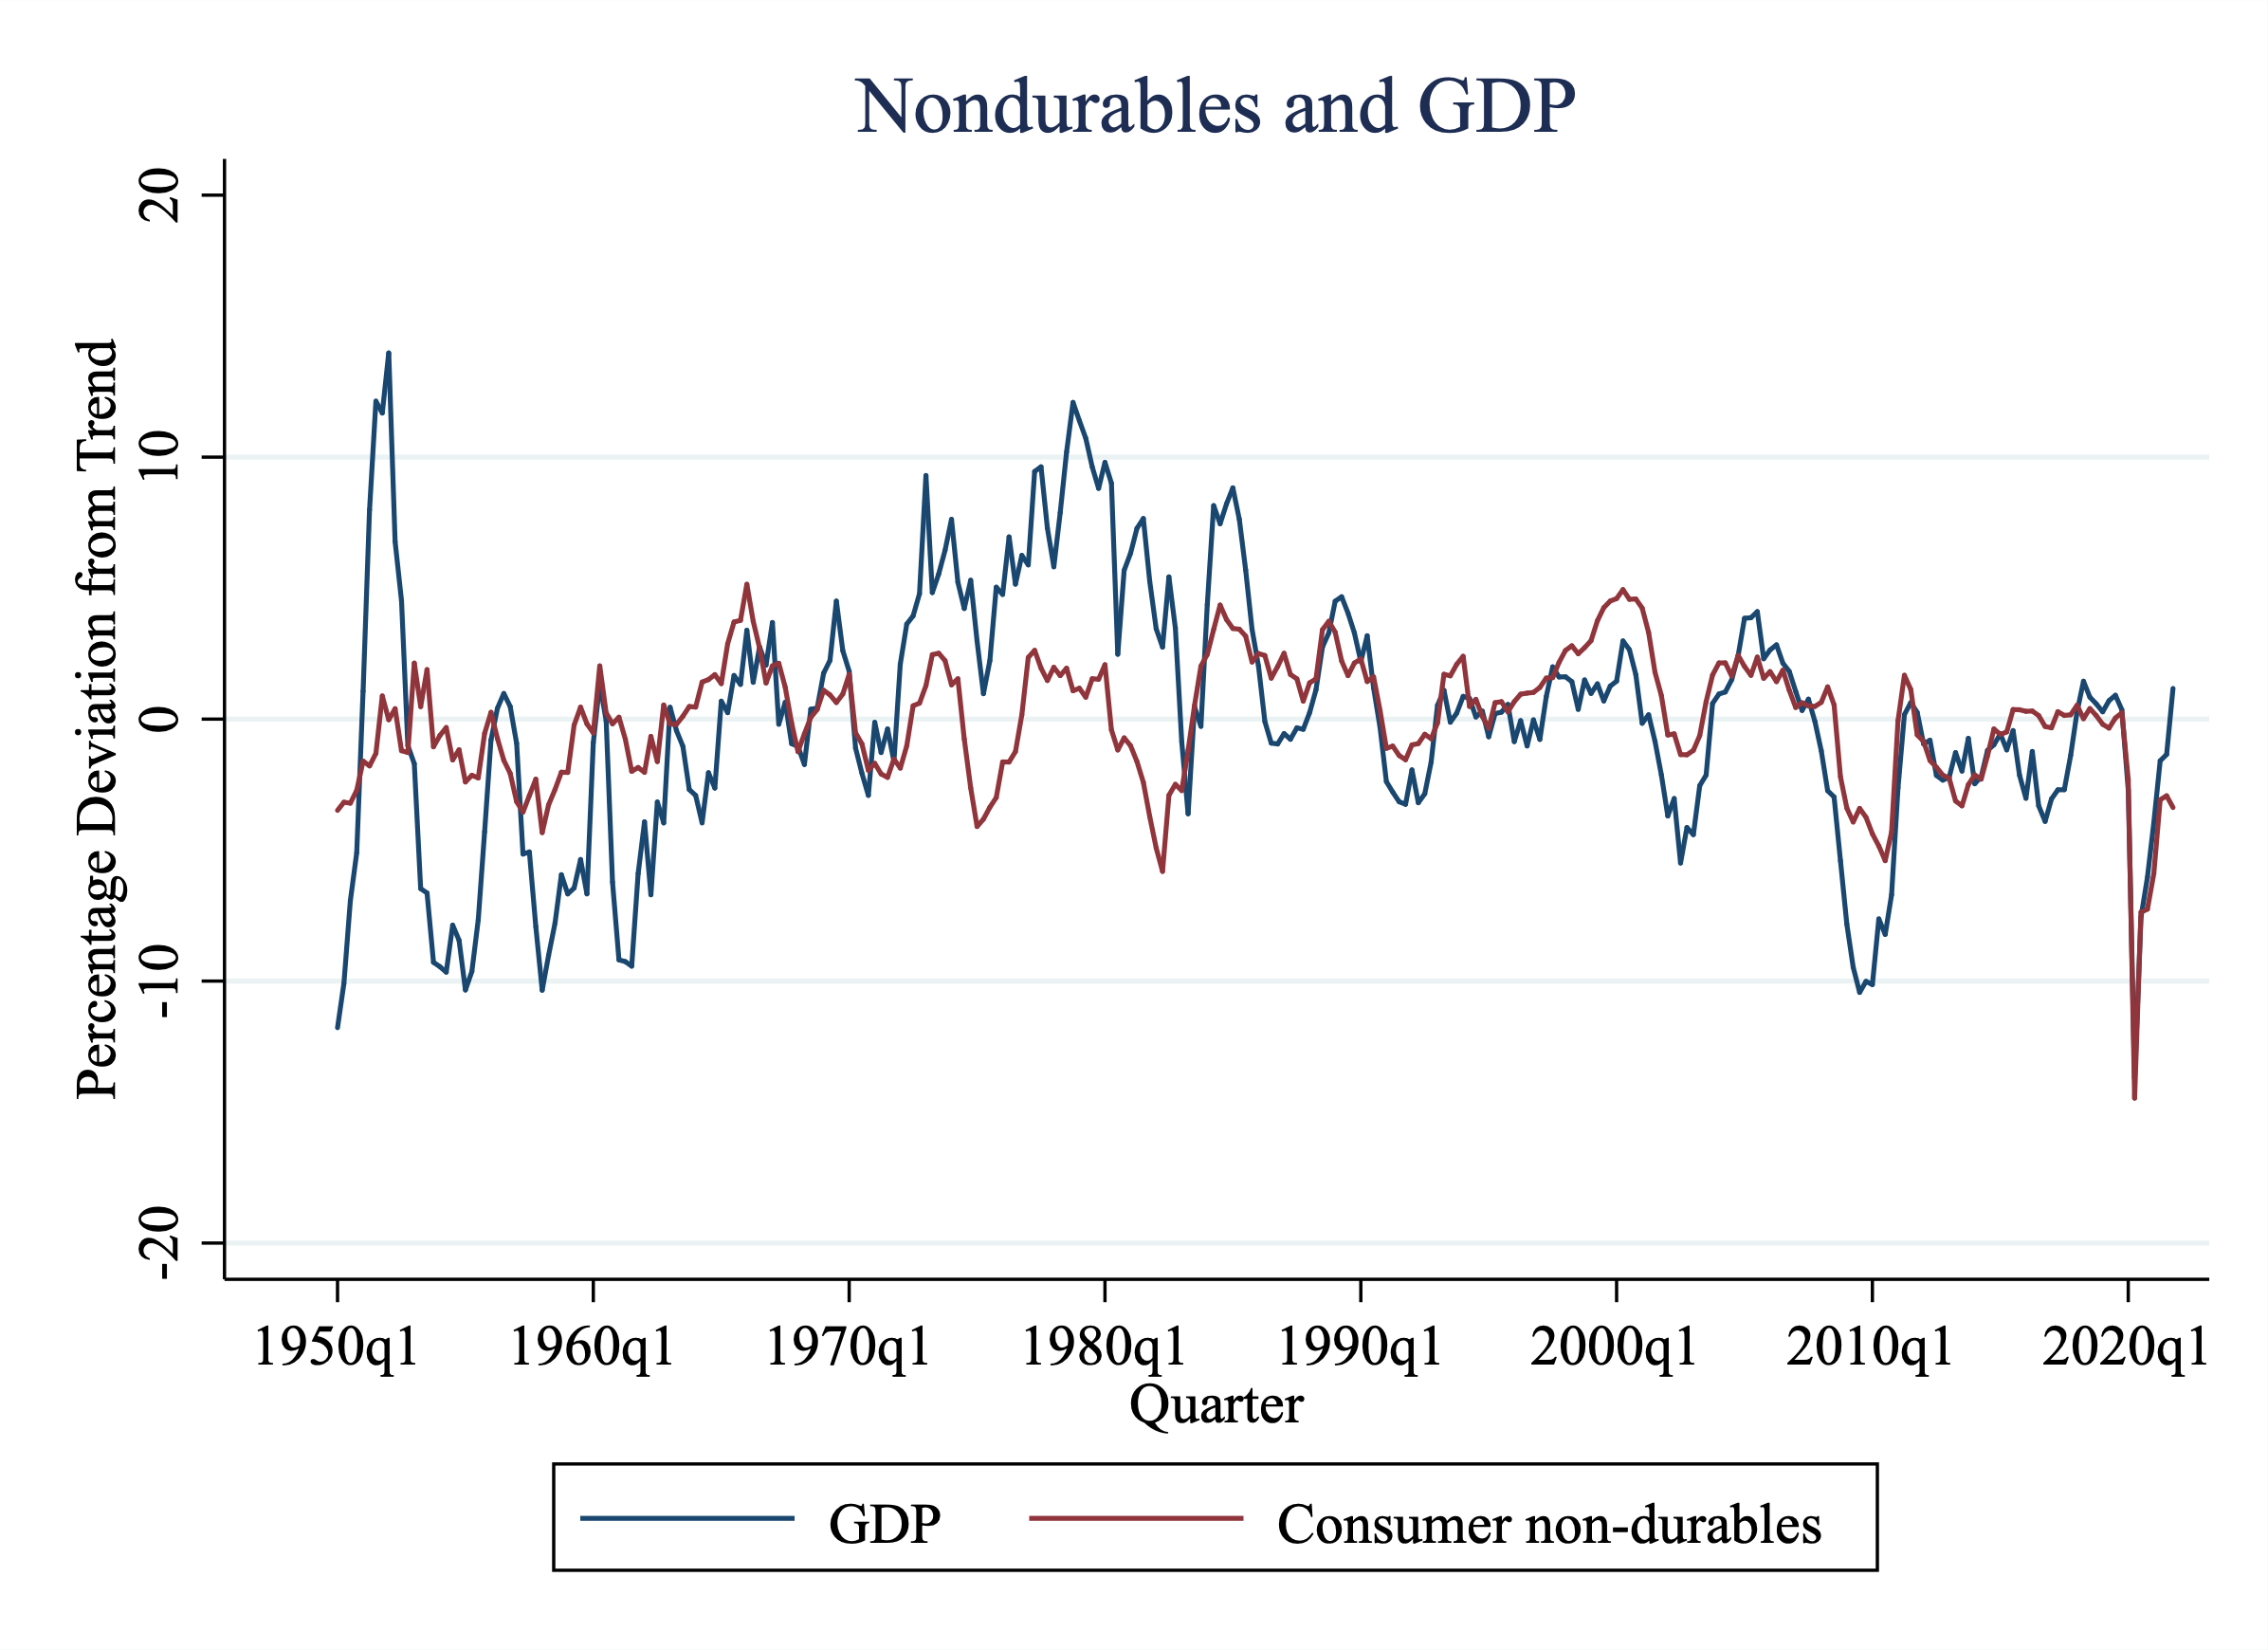
\includegraphics[scale=0.2]{Figures/Fig_9pt7.png}
\end{figure}
Nondurable consumption is less than half as volatile than GDP.  Still, there is excess variablility...
\end{frame}

\begin{frame}
\frametitle[alignment=center]{Excess Variability}
\begin{itemize}
\item Perhaps there are imperfections in the credit market?
\bigskip
\item Or consumers are trying to smooth (borrow when times are bad) and this raises interest rates, causing less smoothing in equilibrium
\end{itemize}
\end{frame}

\begin{frame}
\frametitle[alignment=center]{Increase in future income has same effect on lifetime income as increase in current income!}
\begin{figure}
\centering
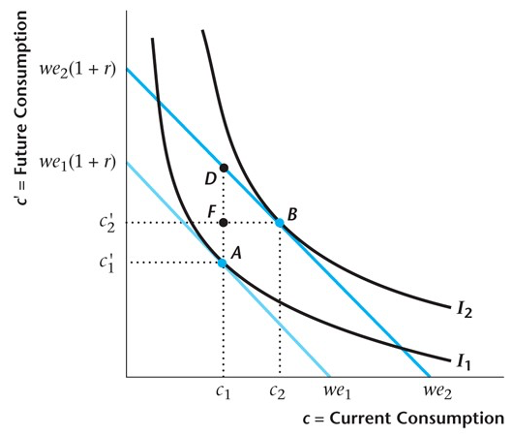
\includegraphics[scale=0.5]{Figures/W_Fig_9pt8.png}
\end{figure}
\end{frame}

\begin{frame}
\frametitle[alignment=center]{Temporary vs permanent changes!}
\begin{figure}
\centering
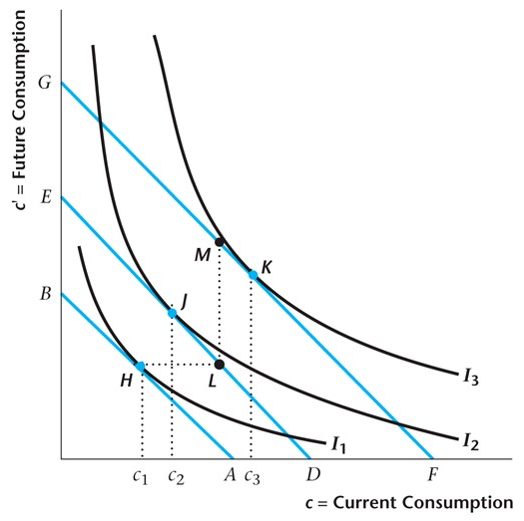
\includegraphics[scale=0.5]{Figures/W_Fig_9pt9.png}
\end{figure}
\end{frame}


\begin{frame}
\frametitle[alignment=center]{Changes in the real interest rate}
\begin{figure}
\centering
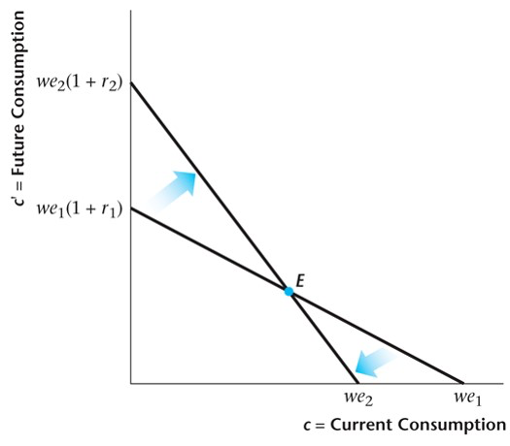
\includegraphics[scale=0.5]{Figures/W_Fig_9pt12.png}
\end{figure}
\end{frame}

\begin{frame}
\frametitle[alignment=center]{Changes in the real interest rate}
\begin{itemize}
\item Thinking about income and substitution effects of a rise in real interest rates
\bigskip
\item Borrower: 
\begin{itemize}
\item  income effect: poorer, so $c\downarrow$, $c'\downarrow$
\item substitution effect: consumption tomorrow ``cheaper", so $c\downarrow$, $c'\uparrow$
\end{itemize}
\item Lender: 
\begin{itemize}
\item  income effect: richer, so $c\uparrow$, $c'\uparrow$
\item substitution effect: consumption tomorrow ``cheaper", so $c\downarrow$, $c'\uparrow$
\end{itemize}
\item Unclear what happens to borrower $c'$, but $c\downarrow$.  Unclear what happens to lender $c$, but $c'\uparrow$.  For both, $c'/c\uparrow$
\end{itemize}
\end{frame}

\begin{frame}
\frametitle[alignment=center]{Changes in the real interest rate: lender}
\begin{figure}
\centering
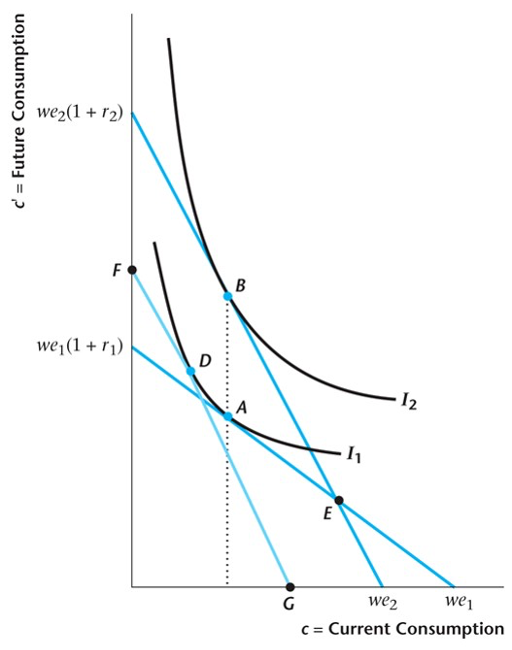
\includegraphics[scale=0.5]{Figures/W_Fig_9pt13.png}
\end{figure}
\end{frame}


\begin{frame}
\frametitle[alignment=center]{Changes in the real interest rate: borrower}
\begin{figure}
\centering
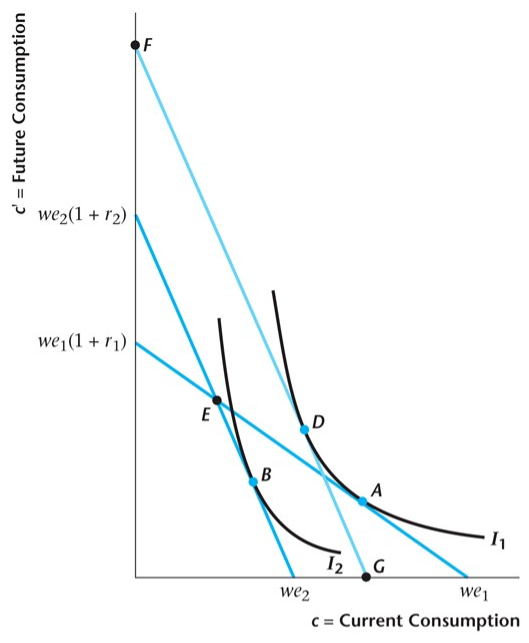
\includegraphics[scale=0.5]{Figures/W_Fig_9pt14.png}
\end{figure}
\end{frame}

\begin{frame}
\frametitle[alignment=center]{Government Budget Constraint}
\begin{itemize}
\item We have the household, now we need a government which can spend on $G$, tax $T$ and borrow $B$:
$$G=T+B$$
$$G+(1+r)B=T'$$
\item Combining the two, we have the government's net present value budget constraint:
$$G+\frac{G}{1+r}=T+\frac{T'}{1+r}$$
\item With this we can combine with the household to get an equilibrium
\end{itemize}
\end{frame}

\begin{frame}
\frametitle[alignment=center]{Equilibrium}
\begin{enumerate}
\item Each consumer chooses optimal first and second period consumption, given $y$, $y'$, and $r$ (HH BC holds)
\bigskip
\item The government present-value budget constraint holds
\bigskip
\item The credit market clears
\end{enumerate}
\end{frame}

\begin{frame}
\frametitle[alignment=center]{Equilibrium in Math}
\begin{itemize}
\item Aggregate private savings must equal government bond holdings in closed economy with no capital:
$$S^P=B$$
\item Total spending is done by households or government:  
$$Y=C+G$$
\item Note that we can derive the second from the first and the private BC:
$$S^P=Y-C-T$$
$$B=G-T$$
\item Plugging in:
$$Y-C-T=G-T$$
$$Y=C+G$$
\item Yay.  
\end{itemize}
\end{frame}

\begin{frame}
\frametitle[alignment=center]{Ricardian Equivalence}
\begin{itemize}
\item If this seems foolish, get ready for a wild prediction!
\smallskip
\item Our model up until now predicts that a lump-sum tax cut with no fall in government savings will not change consumer behavior in the model
\smallskip
\item Take the total tax burden for $N$ consumers:
$$G+\frac{G'}{1+r}=Nt+\frac{Nt'}{1+r}$$
\item Or:
$$t+\frac{t'}{1+r}=\frac{1}{N}\left[G+\frac{G'}{1+r}\right]$$
\item Which we can plug into the consumer's budget constraint:
$$c+\frac{c'}{1+r}=y+\frac{y'}{1+r}-\frac{1}{N}\left[G+\frac{G'}{1+r}\right]$$
\item Implication:  the household doesn't care about when taxation takes place, it only cares about total government spending!
\smallskip
\item If we cut all (lump sum!) taxes today and put them to tomorrow, or vice versa, $c$ and $c'$ shouldn't change!
\end{itemize}
\end{frame}

\begin{frame}
\frametitle[alignment=center]{Ricardian Equivalence: no change in BC, just endowment}
\begin{figure}
\centering
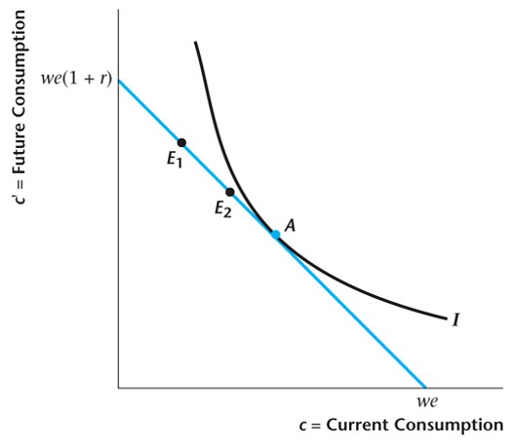
\includegraphics[scale=0.5]{Figures/W_Fig_9pt16.png}
\end{figure}
\end{frame}

\begin{frame}
\frametitle[alignment=center]{Ricardian Equivalence: credit markets}
\begin{figure}
\centering
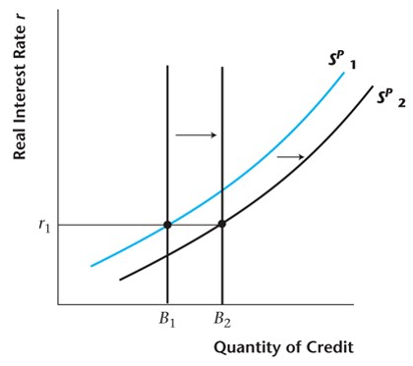
\includegraphics[scale=0.5]{Figures/W_Fig_9pt17.png}
\end{figure}
\end{frame}

\begin{frame}
\frametitle[alignment=center]{Ricardian Equivalence and the Burden of Government Debt}
 We made some assumptions
\begin{itemize}
\item Taxes are not redistributional (between people or across generations)
\bigskip
\item Taxes are lump sum/non-distortionary
\bigskip
\item Credit markets are perfect
\end{itemize}
The point is not that Ricardian Equivalence holds perfectly, but that intertemporal shifts in taxes are filtered through household intertemporal budget constraints
\end{frame}


\begin{frame}
\frametitle[alignment=center]{Federal Government Debt as a Percent of GDP}
 We made some assumptions
\begin{figure}
\centering
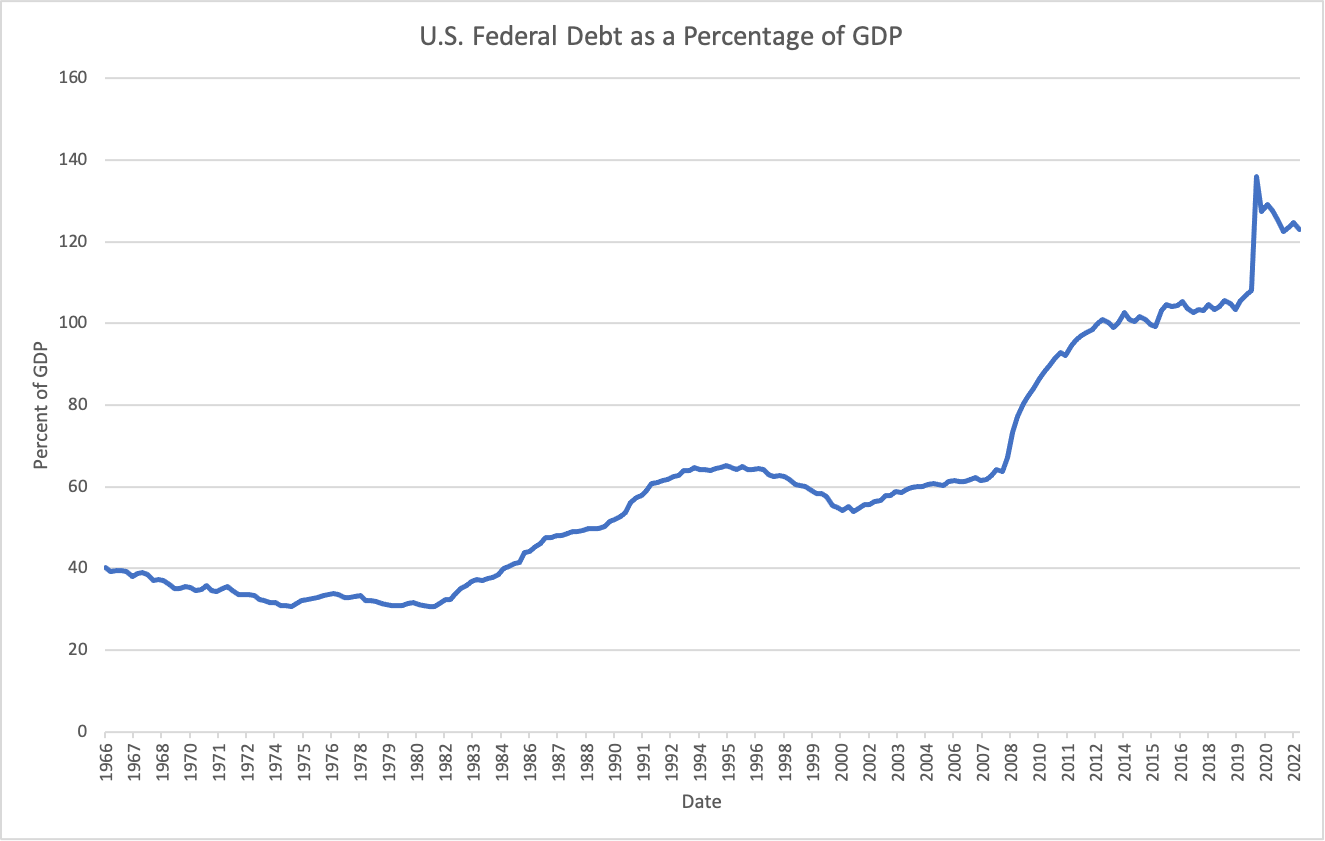
\includegraphics[scale=0.45]{Figures/FedDebt.png}
\end{figure}
\end{frame}


\end{document}